\section*{Problema 3.1}

\textbf{Trabajamos con los de datos fashion MNIST. Ver \url{https://www.kaggle.com/zalando-research/fashionmnist} Se trata de imágenes 28x28 de diez diferentes tipos de prendas. Trabajaremos con \file{fashion-mnist\_train.csv}}

\begin{figure}[H]
    \centering
    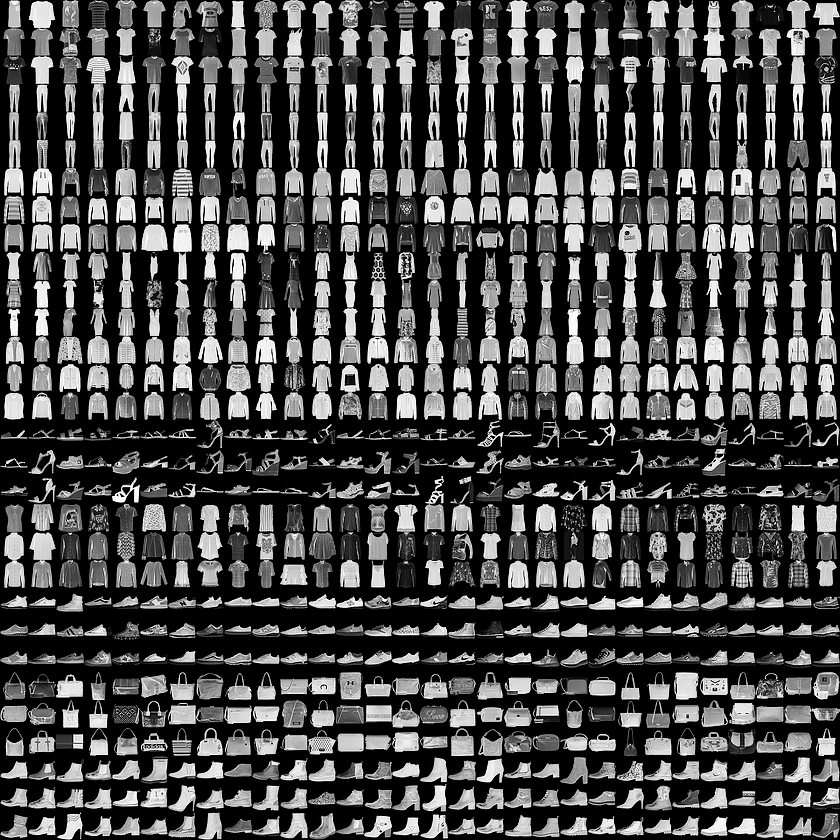
\includegraphics[width=8cm]{Graphics/Problema_3_1.png}
    \caption{}
\end{figure}

\textbf{Busca visualizaciones 2D y 3D basadas en PCA de las imágenes de T-shirts (clase "0`'). ¿ Ves posible encontrar interpretaciones de los componentes como lo hicimos en clase con la base mnist (clásico) de dígitos?}